\documentclass{beamer}

\usetheme{Boadilla}
% \usecolortheme{seahorse}
\usecolortheme{dolphin}
\usefonttheme{serif}

\usepackage{lipsum}
\usepackage{graphicx,xcolor}
\usepackage{amsmath,amssymb,amsfonts}
\usepackage{pgfplots}

% for Chinese
\usepackage{caption}
\usepackage{fontspec}               		% 加這個就可以設定字體
\usepackage[BoldFont, SlantFont]{xeCJK} 	% 讓中英文字體分開設置
\setCJKmainfont{Noto Sans CJK TC}
\setCJKmonofont{Noto Serif CJK TC}

\XeTeXlinebreaklocale "zh" %文字間隔

\XeTeXlinebreakskip = 0pt plus 1pt

\renewcommand{\baselinestretch}{1.4}



\title[Short Title]{Your Title}
% \subtitle{[Course Code] Presentation}
\author[xxxx]{Second Title}
\institute[Group]{Member1, Member2}
\date{20xx.xx.xx}
% \titlegraphic{\includegraphics[width=2cm]{images/logo/iiserm_logo.jpg}}

\begin{document}

\begin{frame}
\titlepage
\end{frame}

\AtBeginSection[]{ 
    \begin{frame}{Table of Contents} 
        \tableofcontents[currentsection] 
    \end{frame} }

\section{Section 1}
\begin{frame}{Section 1}
    \begin{itemize}
        \item List 1
        \begin{itemize}
            \item Description 1
            \item Description 2
            \begin{itemize}
                \item ----
                \item ----
            \end{itemize}
        \end{itemize}
        \item List 2
    \end{itemize}
\end{frame}

\section{Section 2}
\begin{frame}{Section 2}
    \begin{itemize}
        \item Get equation $x = y$
        \begin{itemize}
            \item $x \sim$ Uni$(0, 1)$
            \item \textcolor{blue}{To have a blue color $X_0$}
            \item package: tikz 
                \begin{itemize}
                    \item 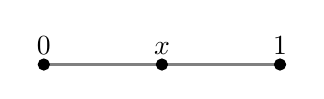
\begin{tikzpicture}
                        \draw[gray, thick] (0, 0) -- (3, 0);
                        \filldraw[black] (0,0) circle (2pt) node[anchor=south]{0};
                        \filldraw[black] (1.5,0) circle (2pt) node[anchor=south]{$x$};
                        \filldraw[black] (3,0) circle (2pt) node[anchor=south]{1};
                    \end{tikzpicture}
                \end{itemize}
        \end{itemize}
    \end{itemize}
\end{frame}


\begin{frame}{Chart}
    \begin{itemize}
        \item To have Objective Function
        \begin{center}
            $\max\limits_{x \geq 0} \ \beta x a^T + (1 - \beta) x a^A$
        \end{center}
        \item To have a Chart
    \end{itemize}
      \\
    \begin{table}[!h]
        \begin{center}
            \begin{tabular}{ c|c|c } 
                    & C & D \\ 
             \hline
             A  & $t_{AC}$   & $t_{AD}$ \\ 
             \hline
             B  & $t_{BC}$   & $t_{BD}$ \\
            \end{tabular}
            \caption*{Table 1}
            % \label{Table 1:}
        \end{center}
    \end{table}
\end{frame}




\section{Section 3}
\begin{frame}{Section 3}
    \begin{columns}
    \column{0.9\textwidth}
        \begin{itemize}
            \item This is section 3 
        \end{itemize}
    \end{columns}
\end{frame}


\section{Section 4}
\begin{frame}{Section 4}
    % \begin{exampleblock}{This is an example block}
    %     \lipsum[5][1-3]
    % \end{exampleblock}
    \begin{itemize}
        \item This is section 4
    \end{itemize}
\end{frame}


\end{document}
